%% report_intermodule_diagram.tex
%% Inter-module communication diagram for the autosoaring PX4 firmware
%% Stock flows: grey dashed arrows
%% New / modified flows: red solid arrows
%% Author: Radhouene
%% Compiler: pdflatex
%%
\documentclass[11pt,a4paper]{article}

\usepackage[T1]{fontenc}
\usepackage[utf8]{inputenc}
\usepackage[margin=2cm]{geometry}
\usepackage{xcolor}
\usepackage{amsmath,amssymb}
\usepackage{booktabs}
\usepackage{graphicx}
\usepackage{parskip}
\usepackage[protrusion=true,expansion=false]{microtype}
\usepackage{hyperref}

% ── TikZ ───────────────────────────────────────────────────────────────────
\usepackage{tikz}
\usetikzlibrary{arrows.meta, positioning, fit, shapes.geometric, calc}

% ── Colour palette ─────────────────────────────────────────────────────────
\definecolor{colNew}{RGB}{200,0,0}       % new additions
\definecolor{colStock}{RGB}{130,130,130} % stock PX4
\definecolor{colMod}{RGB}{220,100,0}     % modified stock
\definecolor{colBox}{RGB}{235,245,255}   % module box fill
\definecolor{colBoxNew}{RGB}{255,235,235}% new module box fill

% ── TikZ styles ────────────────────────────────────────────────────────────
\tikzset{
  module/.style={
    draw, rectangle, rounded corners=4pt,
    fill=colBox, minimum width=3.4cm, minimum height=1.1cm,
    font=\sffamily\small\bfseries, align=center, text width=3.0cm
  },
  newmodule/.style={
    draw=colNew, rectangle, rounded corners=4pt,
    fill=colBoxNew, minimum width=3.4cm, minimum height=1.1cm,
    font=\sffamily\small\bfseries, align=center, text width=3.0cm,
    thick
  },
  stockarr/.style={
    draw=colStock, -{Stealth[length=5pt]}, dashed, line width=0.8pt
  },
  newarr/.style={
    draw=colNew, -{Stealth[length=6pt]}, line width=1.4pt
  },
  modarr/.style={
    draw=colMod, -{Stealth[length=6pt]}, line width=1.2pt, dashed
  },
  topic/.style={
    font=\color{colNew}\ttfamily\tiny, above, midway
  },
  stocktopic/.style={
    font=\color{colStock}\ttfamily\tiny, above, midway
  },
  modtopic/.style={
    font=\color{colMod}\ttfamily\tiny, above, midway
  },
}

% ── Document ───────────────────────────────────────────────────────────────
\title{\textbf{Autosoaring PX4 --- Inter-Module Communication Diagram}\\[4pt]
\large \textcolor{colNew}{$\blacksquare$\rule{0.8cm}{1.5pt}} New flows \quad
       \textcolor{colStock}{- - - - -} Stock PX4 flows \quad
       \textcolor{colMod}{- - - - -} Modified flows}
\author{Radhouene}
\date{\today}

\begin{document}
\maketitle

% ============================================================================
% MAIN DIAGRAM
% ============================================================================
\begin{center}
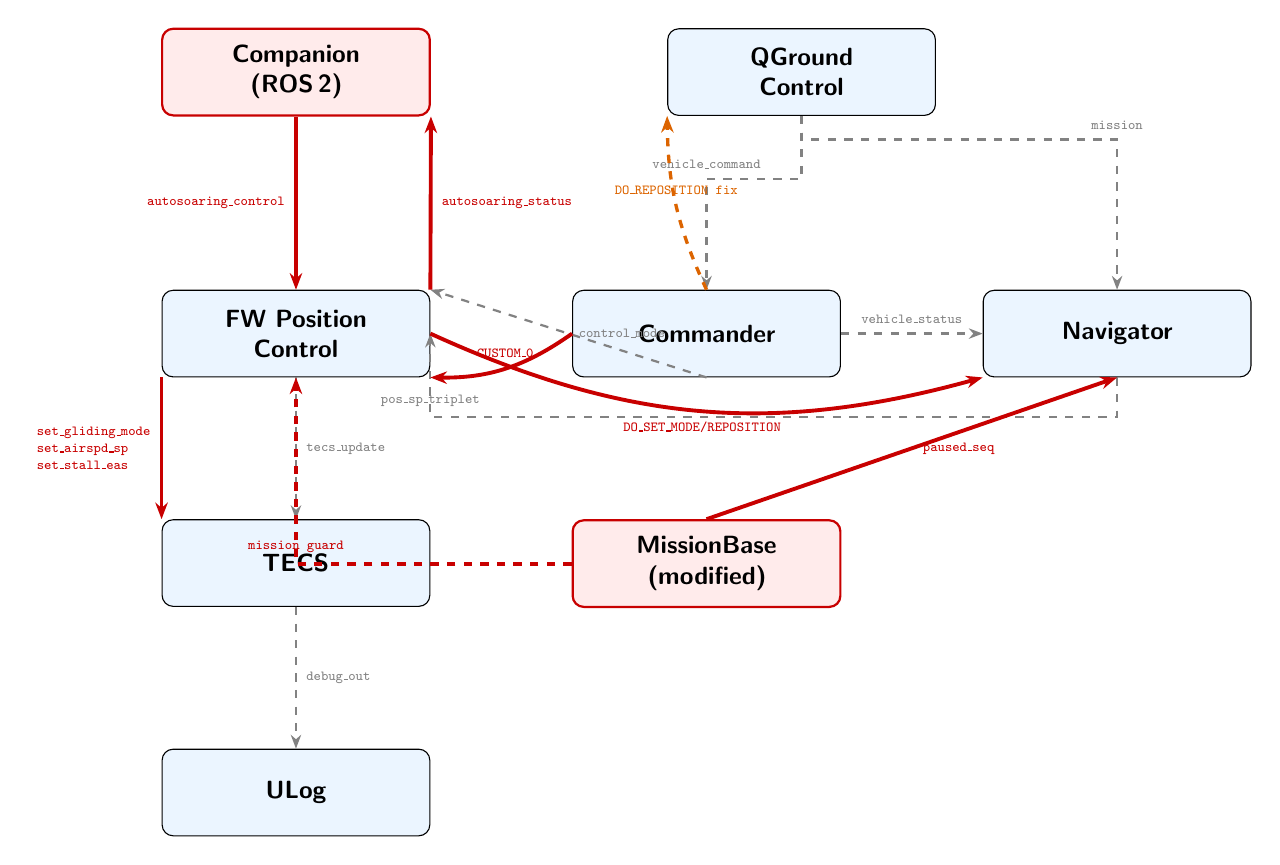
\begin{tikzpicture}[node distance=1.4cm and 1.8cm]

% ── Nodes ──────────────────────────────────────────────────────────────────
% Row 1 (top): external actors
\node[newmodule]  (companion) {Companion\\(ROS\,2)};
\node[module, right=3.0cm of companion] (qgc) {QGround\\Control};

% Row 2: FMU modules
\node[module, below=2.2cm of companion] (fwpos) {FW Position\\Control};
\node[module, right=1.8cm of fwpos]     (commander) {Commander};
\node[module, right=1.8cm of commander] (navigator) {Navigator};

% Row 3: inner lib
\node[module, below=1.8cm of fwpos]    (tecs) {TECS};
\node[newmodule, below=1.8cm of commander] (mbase) {MissionBase\\(modified)};

% Row 4: ulog/debug
\node[module, below=1.8cm of tecs]     (ulog) {ULog};

% ── Stock flows ─────────────────────────────────────────────────────────────
% QGC → Commander
\draw[stockarr] (qgc.south) -- ++(0,-0.8) -| node[stocktopic]{vehicle\_command} (commander.north);

% Commander → Navigator
\draw[stockarr] (commander.east) -- node[stocktopic]{vehicle\_status} (navigator.west);

% Commander → fw_pos_ctrl
\draw[stockarr] (commander.south) -- node[stocktopic, right]{control\_mode} (fwpos.north east);

% Navigator → fw_pos_ctrl
\draw[stockarr] (navigator.south) -- ++(0,-0.5) -| node[stocktopic]{pos\_sp\_triplet} (fwpos.east);

% fw_pos_ctrl → TECS
\draw[stockarr] (fwpos.south) -- node[stocktopic, right]{tecs\_update} (tecs.north);

% TECS → ULog
\draw[stockarr] (tecs.south) -- node[stocktopic, right]{debug\_out} (ulog.north);

% QGC → Navigator
\draw[stockarr] (qgc.south) -- ++(0,-0.3) -| node[stocktopic]{mission} (navigator.north);

% ── New flows (red) ─────────────────────────────────────────────────────────
% Companion → fw_pos_ctrl
\draw[newarr] (companion.south) -- node[topic, left]{\textbf{autosoaring\_control}} (fwpos.north);

% fw_pos_ctrl → Companion
\draw[newarr] (fwpos.north east) -- node[topic, right]{\textbf{autosoaring\_status}} (companion.south east);

% Commander → fw_pos_ctrl (CUSTOM_0)
\draw[newarr, bend left=18] (commander.west) to node[topic, above]{\textbf{CUSTOM\_0}} (fwpos.south east);

% fw_pos_ctrl → Navigator (DO_SET_MODE, DO_REPOSITION)
\draw[newarr, bend right=20] (fwpos.east) to node[topic, below]{\textbf{DO\_SET\_MODE/REPOSITION}} (navigator.south west);

% fw_pos_ctrl → TECS (new setters)
\draw[newarr] (fwpos.south west) -- node[topic, left, align=left]{set\_gliding\_mode\\set\_airspd\_sp\\set\_stall\_eas} (tecs.north west);

% MissionBase → Navigator
\draw[newarr] (mbase.north) -- node[topic, right]{\textbf{paused\_seq}} (navigator.south);

% MissionBase → fw_pos_ctrl (mission sub)
\draw[newarr, dashed] (mbase.west) -| node[topic]{\textbf{mission guard}} (fwpos.south);

% ── Modified flows (orange) ──────────────────────────────────────────────────
\draw[modarr, bend left=12] (commander.north) to node[modtopic]{\textbf{DO\_REPOSITION fix}} (qgc.south west);

% (Background group boxes removed to avoid LaTeX scope conflicts)

\end{tikzpicture}
\end{center}

\vspace{1em}

% ============================================================================
% LEGEND TABLE
% ============================================================================
\begin{center}
\begin{tabular}{lll}
\toprule
Colour & Style & Meaning \\
\midrule
\textcolor{colNew}{\rule{1.2cm}{2pt}} & Solid & \textbf{New} flow added for autosoaring \\
\textcolor{colStock}{\tikz{\draw[dashed,colStock,line width=0.8pt](0,0)--(1.2cm,0);}} & Dashed & Stock PX4 flow (unchanged) \\
\textcolor{colMod}{\tikz{\draw[dashed,colMod,line width=1pt](0,0)--(1.2cm,0);}} & Dashed orange & \textbf{Modified} stock flow \\
\bottomrule
\end{tabular}
\end{center}

\newpage

% ============================================================================
% VARIABLE MAP TABLE
% ============================================================================
\section*{Key Variables and Messages Between Modules}

\begin{center}
\renewcommand{\arraystretch}{1.35}
\begin{tabular}{p{4.8cm}p{2.8cm}p{2.8cm}p{5.5cm}}
\toprule
Variable / Topic & Publisher & Subscriber(s) & Role \\
\midrule
\multicolumn{4}{l}{\textit{\textcolor{colNew}{--- New (autosoaring) ---}}} \\
\texttt{autosoaring\_control} uORB & Companion / ROS\,2 & \texttt{fw\_pos\_control} & Soaring mode, loiter centre, bank angle, airspeed cmd \\
\texttt{autosoaring\_status} uORB & \texttt{fw\_pos\_control} & Companion / ROS\,2 & FMU feedback: mode effective, DDS inhibit expiry, FMU phase \\
\texttt{VEHICLE\_CMD\_CUSTOM\_0} & Commander (CLI) & \texttt{fw\_pos\_control} & CLI soaring mode 0--4 with optional bank/radius \\
\texttt{VEHICLE\_CMD\_DO\_REPOSITION} & \texttt{fw\_pos\_control} & Navigator & Thermal loiter centre pin \\
\texttt{VEHICLE\_CMD\_DO\_SET\_MODE} (heartbeat) & \texttt{fw\_pos\_control} & Commander & Keep AUTO\_MISSION while gliding (1\,s refresh) \\
\texttt{set\_gliding\_mode\_enabled()} & \texttt{fw\_pos\_control} & TECS & Toggle engine-off control path \\
\texttt{set\_gliding\_airspeed\_setpoint()} & \texttt{fw\_pos\_control} & TECS & Pre-computed EAS (fixed / polar) \\
\texttt{set\_glide\_stall\_eas()} & \texttt{fw\_pos\_control} & TECS & Glide floor from \texttt{FW\_AIRSPD\_STALL} \\
\texttt{set\_glide\_i\_decay()} & \texttt{fw\_pos\_control} & TECS & Throttle integrator decay constant \\
\texttt{\_mission\_paused\_seq} & \texttt{MissionBase} & \texttt{MissionBase} (internal) & Clamp stale uORB seq during AUTO\_LOITER \\
\texttt{\_soaring\_local\_override} & \texttt{vehicle\_command\_poll} & \texttt{Run()} DDS poll & CLI authority flag \\
\texttt{\_soaring\_dds\_inhibit\_until\_us} & \texttt{vehicle\_command\_poll} & \texttt{Run()} DDS poll & 5\,s DDS cooldown after soar:off \\
\midrule
\multicolumn{4}{l}{\textit{--- Stock PX4 (unchanged) ---}} \\
\texttt{vehicle\_status} & Commander & Navigator, \texttt{fw\_pos\_control} & nav\_state, vehicle type \\
\texttt{vehicle\_control\_mode} & Commander & \texttt{fw\_pos\_control} & Flags: auto, position, armed, … \\
\texttt{position\_setpoint\_triplet} & Navigator & \texttt{fw\_pos\_control} & Waypoints (type, lat, lon, alt, radius) \\
\texttt{mission} & GCS / dataman & Navigator, \texttt{fw\_pos\_control} & Mission items and current seq \\
\texttt{vehicle\_command} (general) & GCS/MAVLink & Commander, Navigator & Arm, calibrate, mode switch \\
\bottomrule
\end{tabular}
\end{center}

\newpage

% ============================================================================
% AUTHORITY ARBITRATION DIAGRAM
% ============================================================================
\section*{Authority Arbitration Flow (fw\_pos\_control DDS Poll)}

\begin{center}
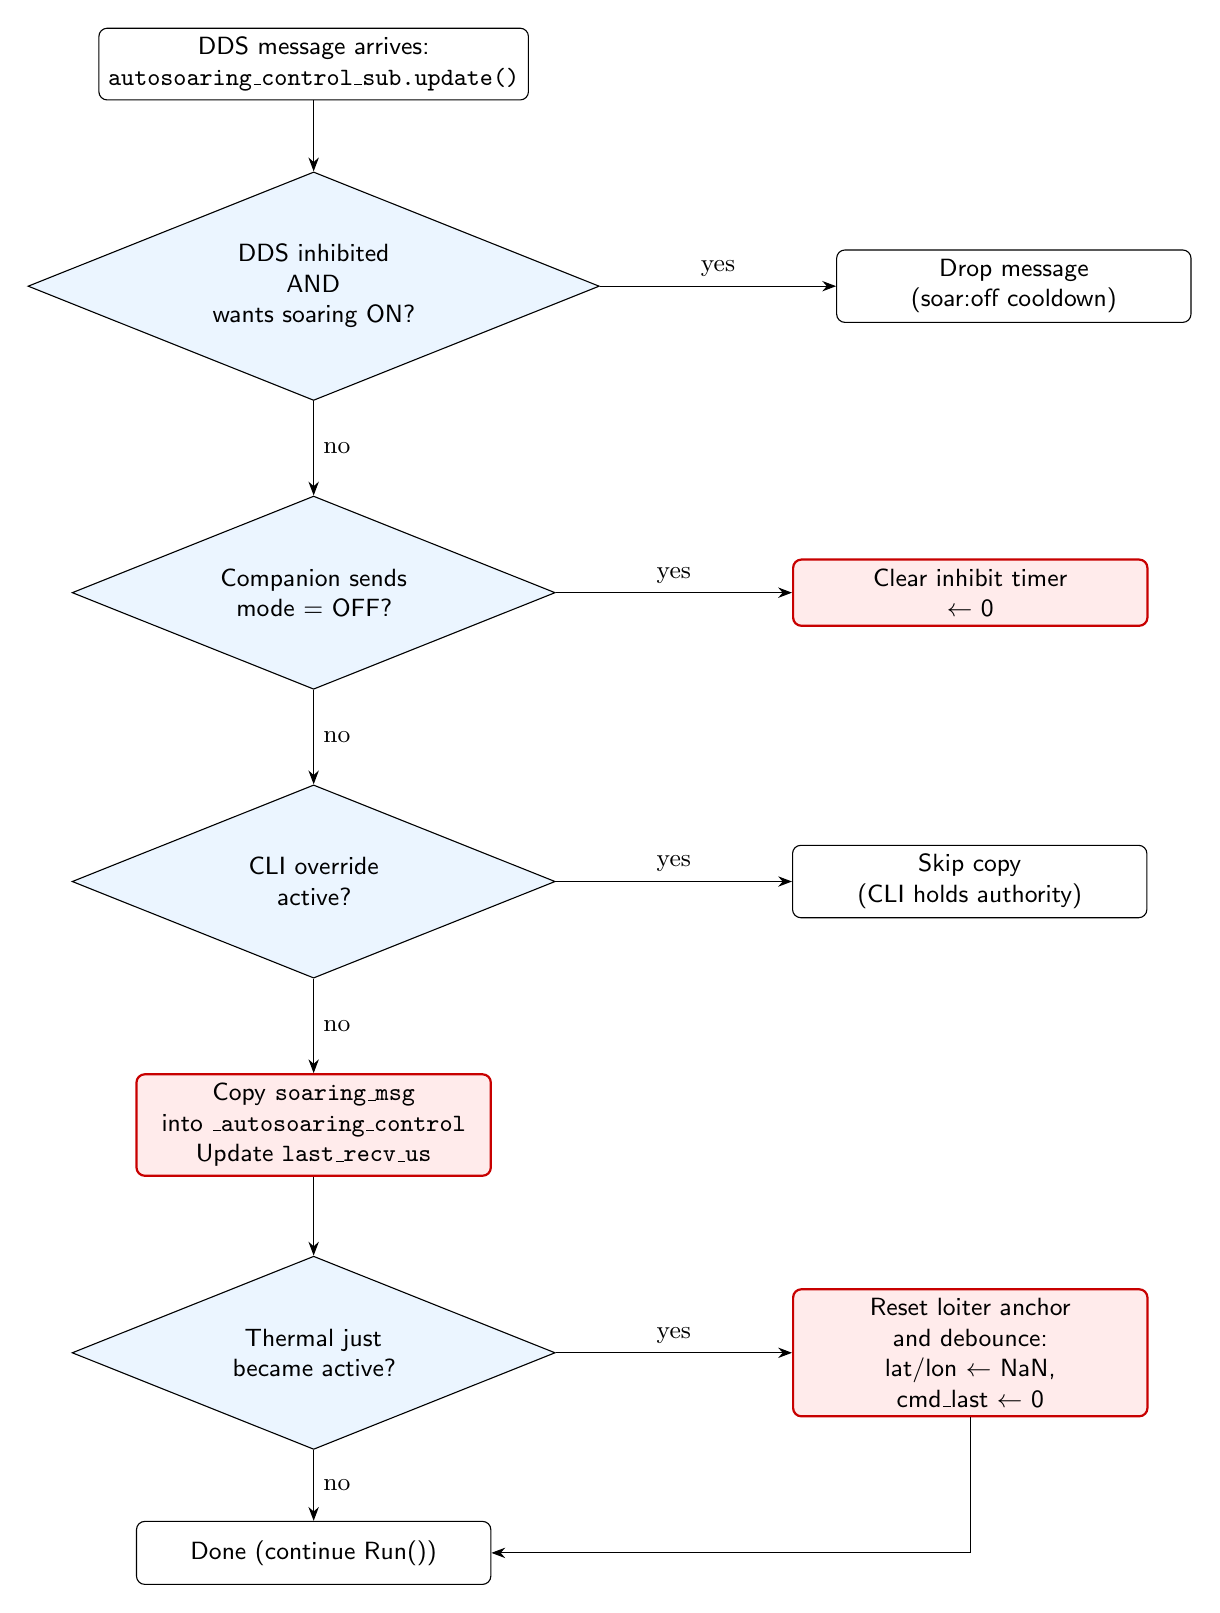
\begin{tikzpicture}[
  node distance=1.4cm,
  decision/.style={diamond, draw, fill=colBox, aspect=2.5,
                   font=\sffamily\small, align=center, text width=3.8cm},
  action/.style={rectangle, rounded corners=3pt, draw,
                 font=\sffamily\small, align=center, minimum width=4.5cm,
                 minimum height=0.8cm},
  newact/.style={rectangle, rounded corners=3pt, draw=colNew, fill=colBoxNew,
                 font=\sffamily\small, align=center, minimum width=4.5cm,
                 minimum height=0.8cm, thick},
  arr/.style={{Stealth[length=5pt]}-, line width=0.9pt},
  narr/.style=-{Stealth[length=5pt]},
]

\node[action] (start) {DDS message arrives:\\
  \texttt{autosoaring\_control\_sub.update()}};

\node[decision, below=0.9cm of start] (inh) {DDS inhibited\\AND\\wants soaring ON?};
\node[action, right=3cm of inh]  (drop) {Drop message\\\small(soar:off cooldown)};

\node[decision, below=1.2cm of inh] (clr) {Companion sends\\mode = OFF?};
\node[newact, right=3cm of clr]   (clrinh) {Clear inhibit timer\\$\leftarrow$ 0};

\node[decision, below=1.2cm of clr] (ovr) {CLI override\\active?};
\node[action, right=3cm of ovr]   (skip) {Skip copy\\\small(CLI holds authority)};

\node[newact, below=1.2cm of ovr]  (copy) {Copy \texttt{soaring\_msg}\\into \texttt{\_autosoaring\_control}\\Update \texttt{last\_recv\_us}};

\node[decision, below=1.0cm of copy] (newth) {Thermal just\\became active?};
\node[newact, right=3cm of newth]  (reset) {Reset loiter anchor\\and debounce:\\ lat/lon $\leftarrow$ NaN,\\ cmd\_last $\leftarrow$ 0};

\node[action, below=0.9cm of newth] (done) {Done (continue Run())};

% arrows
\draw[narr] (start) -- (inh);
\draw[narr] (inh.east) -- node[above]{\small yes} (drop.west);
\draw[narr] (inh.south) -- node[right]{\small no} (clr.north);
\draw[narr] (clr.east) -- node[above]{\small yes} (clrinh.west);
\draw[narr] (clr.south) -- node[right]{\small no} (ovr.north);
\draw[narr] (ovr.east) -- node[above]{\small yes} (skip.west);
\draw[narr] (ovr.south) -- node[right]{\small no} (copy.north);
\draw[narr] (copy.south) -- (newth.north);
\draw[narr] (newth.east) -- node[above]{\small yes} (reset.west);
\draw[narr] (newth.south) -- node[right]{\small no} (done.north);
\draw[narr] (reset.south) |- (done.east);

\end{tikzpicture}
\end{center}

\vspace{0.5em}
\noindent
\textcolor{colNew}{\textbf{Red / orange boxes}} are new logic; white boxes are stock PX4 handling.
The \textbf{CLI override flag} (\texttt{\_soaring\_local\_override}) is the primary
gate: when \texttt{true}, the DDS copy is skipped entirely regardless of the inhibit
timer.

\end{document}
